% Canonical manuscript source. The older Pandoc Markdown draft was archived in
% ../archive/2026-04-03-markdown-source/gut_application_paper.md.
% Options for packages loaded elsewhere
\PassOptionsToPackage{unicode}{hyperref}
\PassOptionsToPackage{hyphens}{url}
\PassOptionsToPackage{dvipsnames,svgnames,x11names}{xcolor}
\documentclass[
  11pt,
]{article}
\usepackage{xcolor}
\usepackage[margin=1in]{geometry}
\usepackage{amsmath,amssymb}
\setcounter{secnumdepth}{-\maxdimen} % remove section numbering
\usepackage{iftex}
\ifPDFTeX
  \usepackage[T1]{fontenc}
  \usepackage[utf8]{inputenc}
  \usepackage{textcomp} % provide euro and other symbols
\else % if luatex or xetex
  \usepackage{unicode-math} % this also loads fontspec
  \defaultfontfeatures{Scale=MatchLowercase}
  \defaultfontfeatures[\rmfamily]{Ligatures=TeX,Scale=1}
\fi
\usepackage{lmodern}
\ifPDFTeX\else
  % xetex/luatex font selection
\fi
% Use upquote if available, for straight quotes in verbatim environments
\IfFileExists{upquote.sty}{\usepackage{upquote}}{}
\IfFileExists{microtype.sty}{% use microtype if available
  \usepackage[]{microtype}
  \UseMicrotypeSet[protrusion]{basicmath} % disable protrusion for tt fonts
}{}
\usepackage{setspace}
\makeatletter
\@ifundefined{KOMAClassName}{% if non-KOMA class
  \IfFileExists{parskip.sty}{%
    \usepackage{parskip}
  }{% else
    \setlength{\parindent}{0pt}
    \setlength{\parskip}{6pt plus 2pt minus 1pt}}
}{% if KOMA class
  \KOMAoptions{parskip=half}}
\makeatother
\usepackage{longtable,booktabs,array}
\usepackage{calc} % for calculating minipage widths
% Correct order of tables after \paragraph or \subparagraph
\usepackage{etoolbox}
\makeatletter
\patchcmd\longtable{\par}{\if@noskipsec\mbox{}\fi\par}{}{}
\makeatother
% Allow footnotes in longtable head/foot
\IfFileExists{footnotehyper.sty}{\usepackage{footnotehyper}}{\usepackage{footnote}}
\makesavenoteenv{longtable}
\usepackage{graphicx}
\makeatletter
\newsavebox\pandoc@box
\newcommand*\pandocbounded[1]{% scales image to fit in text height/width
  \sbox\pandoc@box{#1}%
  \Gscale@div\@tempa{\textheight}{\dimexpr\ht\pandoc@box+\dp\pandoc@box\relax}%
  \Gscale@div\@tempb{\linewidth}{\wd\pandoc@box}%
  \ifdim\@tempb\p@<\@tempa\p@\let\@tempa\@tempb\fi% select the smaller of both
  \ifdim\@tempa\p@<\p@\scalebox{\@tempa}{\usebox\pandoc@box}%
  \else\usebox{\pandoc@box}%
  \fi%
}
% Set default figure placement to htbp
\def\fps@figure{htbp}
\makeatother
% definitions for citeproc citations
\NewDocumentCommand\citeproctext{}{}
\NewDocumentCommand\citeproc{mm}{%
  \begingroup\def\citeproctext{#2}\cite{#1}\endgroup}
\makeatletter
 % allow citations to break across lines
 \let\@cite@ofmt\@firstofone
 % avoid brackets around text for \cite:
 \def\@biblabel#1{}
 \def\@cite#1#2{{#1\if@tempswa , #2\fi}}
\makeatother
\newlength{\cslhangindent}
\setlength{\cslhangindent}{1.5em}
\newlength{\csllabelwidth}
\setlength{\csllabelwidth}{3em}
\newenvironment{CSLReferences}[2] % #1 hanging-indent, #2 entry-spacing
 {\begin{list}{}{%
  \setlength{\itemindent}{0pt}
  \setlength{\leftmargin}{0pt}
  \setlength{\parsep}{0pt}
  % turn on hanging indent if param 1 is 1
  \ifodd #1
   \setlength{\leftmargin}{\cslhangindent}
   \setlength{\itemindent}{-1\cslhangindent}
  \fi
  % set entry spacing
  \setlength{\itemsep}{#2\baselineskip}}}
 {\end{list}}
\usepackage{calc}
\newcommand{\CSLBlock}[1]{\hfill\break\parbox[t]{\linewidth}{\strut\ignorespaces#1\strut}}
\newcommand{\CSLLeftMargin}[1]{\parbox[t]{\csllabelwidth}{\strut#1\strut}}
\newcommand{\CSLRightInline}[1]{\parbox[t]{\linewidth - \csllabelwidth}{\strut#1\strut}}
\newcommand{\CSLIndent}[1]{\hspace{\cslhangindent}#1}
\setlength{\emergencystretch}{3em} % prevent overfull lines
\providecommand{\tightlist}{%
  \setlength{\itemsep}{0pt}\setlength{\parskip}{0pt}}
\usepackage{booktabs}
\usepackage{longtable}
\usepackage{array}
\usepackage{tabularx}
\usepackage{float}
\usepackage{titling}
\usepackage{caption}
\captionsetup{font=small,labelfont=bf}
\newcolumntype{Y}{>{\raggedright\arraybackslash}X}
\newcommand{\taxon}[1]{\emph{#1}}
\newcommand{\dcstsep}{/\allowbreak}
\setlength{\droptitle}{-2.6em}
\pretitle{\begin{center}\Large}
\posttitle{\par\end{center}\vspace{0.55em}}
\preauthor{\begin{center}\normalsize}
\postauthor{\par\end{center}\vspace{-0.5em}}
\predate{}
\postdate{}
\usepackage{bookmark}
\IfFileExists{xurl.sty}{\usepackage{xurl}}{} % add URL line breaks if available
\urlstyle{same}
\hypersetup{
  pdftitle={Dominant Community State Types Reveal Disease-Associated Dominance Patterns in the Human Gut Microbiome},
  colorlinks=true,
  linkcolor={blue},
  filecolor={Maroon},
  citecolor={Blue},
  urlcolor={blue},
  pdfcreator={LaTeX via pandoc}}
\newcommand{\paperaffiliation}{Center for Advanced Microbiome Research and Innovation (CAMRI), Institute for Genome Sciences, Department of Microbiology and Immunology, University of Maryland School of Medicine, Baltimore, Maryland, USA.}
\newcommand{\paperfundingnote}{Research reported in this publication was supported by grant number INV-048956 from the Gates Foundation.}
\newcommand{\blfootnote}[1]{%
  \begingroup
  \renewcommand{\thefootnote}{}\footnote{#1}%
  \addtocounter{footnote}{-1}%
  \endgroup
}

\title{Dominant Community State Types Reveal Disease-Associated
Dominance Patterns in the Human Gut Microbiome}
\author{\parbox{0.9\textwidth}{\centering Pawel Gajer\thanks{\paperaffiliation}\thanks{Corresponding author: pgajer@gmail.com} and Jacques Ravel\protect\footnotemark[1]}}
\date{}
\newif\ifshowbuildstamp
\showbuildstampfalse
\providecommand{\manuscriptversion}{unversioned}
\providecommand{\manuscriptbuildnumber}{NA}
\providecommand{\manuscriptcommit}{unknown}
\providecommand{\manuscriptbuilddatetime}{unknown}
\InputIfFileExists{../build/manuscript_build_info.tex}{}{}

\begin{document}
\maketitle
\blfootnote{\paperfundingnote}
\ifshowbuildstamp
\begin{center}
\footnotesize
Version \texttt{\manuscriptversion} \quad | \quad Build
\texttt{\manuscriptbuildnumber} \quad | \quad Commit
\texttt{\manuscriptcommit}\\
Built \manuscriptbuilddatetime
\end{center}
\vspace{0.35em}
\fi

\setstretch{1.15}
\section{Abstract}\label{abstract}

Gut microbiome community typing is often cluster based, which makes the
resulting labels sensitive to modeling choices and harder to interpret
sample by sample. We evaluated dominant-community state types (DCSTs),
a deterministic rank-based alternative, in 30,290 quality-controlled
American Gut Project stool samples drawn from a 34,711-sample SILVA
species-level table, using an absorb policy that merges very small
dominance patterns into larger named states. The resulting hierarchy
contained 40 absorb states at depth 1, 153 at depth 2, 479 at depth 3,
and 744 at depth 4. We first screened phenotype-by-depth tables with
adaptive Fisher exact tests and then used both conventional and
Bayesian follow-up models to estimate state-specific enrichment or
depletion. The strongest and most biologically coherent branch was IBD,
and the main text therefore centers on inflammatory phenotypes. IBD showed the strongest structure,
with a broad \taxon{Bacteroides} signal at depth 1 and progressively
stronger \taxon{Bacteroides}-centered lineages at depths 2 to 4; the
Bayesian analysis also highlighted rare enterobacterial states such as
\taxon{Morganella}. IBS showed a milder
\taxon{Escherichia-Shigella}-centered pattern together with depletion of
\taxon{Faecalibacterium}- and \taxon{Prevotella\_9}-linked states.
Autoimmune disease showed a parallel inflammatory pattern centered on
\taxon{Bacteroides} and its deeper lineages. Across the main-text
phenotype branches, Bayesian estimates closely tracked the
conventional adjusted odds ratios while remaining informative for rarer
deeper states. External validation then separated framework
reproducibility from exact label portability: Halfvarson 2017 supported
the IBD branch strongly in both rebuilt-cohort and frozen-transfer
analyses, PRJEB84421 provided narrower rebuilt inflammatory support, and
pooled HMP2 retained a weaker transferred depth-2 IBD signal after
explicit case coding. Together, these results support absorb DCSTs as a
practical, biologist-readable framework for large-scale microbiome
association screens while indicating that exact label transfer remains
strongest in selected inflammatory cohorts rather than universal across
all settings. Additional non-IBD branches are summarized in the
supplement as exploratory extensions of the main inflammatory story.

\textbf{Keywords:} gut microbiome; community typing; dominant-community
state types; American Gut Project; inflammatory bowel disease; Bayesian
modeling

\section{Introduction}\label{introduction}

Microbiome community typing is valuable when it compresses a
high-dimensional abundance profile into a smaller number of biologically
interpretable states. In practice, however, many typing schemes are
built around clustering. That strategy can be informative, but it also
ties the final labels to choices about transformations, distance
metrics, initialization, model class, and the number of clusters. Those
choices affect whether a reader can understand what a given sample label
means and whether two analyses can be compared without a hidden
dependence on tuning decisions.

Here we evaluate a simpler deterministic representation: a dominant-community
state type (DCST), defined by the within-sample ordering of taxa. At depth 1,
the state is assigned by the dominant taxon; at depth 2, it is refined by the
ordered pair of the two most abundant taxa. Because assignment depends only on
within-sample rank order, the same label is recovered from counts, proportions,
or any sample-wide order-preserving normalization. DCSTs therefore provide
explicit, hierarchical sample-level states that can be read directly from the
data, rather than inferred from a fitted global partition. The underlying
pure dCST construct is simply this ordered dominant label itself. In the
present manuscript, we focus on an absorb refinement that merges very
small branches into larger named states so that deeper associations can
be followed without losing interpretability.

We apply this framework to the gut microbiome, where literature on IBS,
IBD, autoimmune disease, and cardiometabolic conditions suggests that
shifts in dominant taxa or dominant taxon pairs can mark altered
ecological states
(\citeproc{ref-Tap2017_IBS}{Tap et al. 2017};
\citeproc{ref-Pittayanon2019_IBS}{Pittayanon et al. 2019};
\citeproc{ref-LloydPrice2019_IBD}{Lloyd-Price et al. 2019};
\citeproc{ref-Gevers2014_CD}{Gevers et al. 2014};
\citeproc{ref-Scher2013_Prevotella_RA}{Scher et al. 2013};
\citeproc{ref-Vatanen2018_T1D}{Vatanen et al. 2018};
\citeproc{ref-Wang2011_TMAO}{Z. Wang et al. 2011};
\citeproc{ref-Tang2013_TMAO}{Tang et al. 2013}). In this setting,
DCSTs provide a natural high-level characterization of community
structure and a useful first abstraction layer for downstream
mechanistic analyses.

Our aim is not to argue that dominant taxa alone explain disease
biology. Rather, we ask whether recurrent dominance patterns can be
identified deterministically in a cohort of this size, whether the
resulting labels retain enough ecological meaning to support
phenotype-specific association screening, and whether the strongest
signals remain biologically readable after covariate adjustment, deeper
hierarchical refinement, and cross-cohort evaluation. If so, DCSTs
provide a practical
analysis layer for large microbiome studies in which interpretability
and reproducibility matter as much as statistical association strength.
In this study we use the
\texttt{absorb} low-frequency policy, which merges very small
dominance patterns into larger named states rather than pooling them
into one catch-all rare category, and we complement standard
association tests with Bayesian models that remain informative for
rarer deeper states. Pure dCST results are used only as a baseline
comparison in the supplement rather than as a second main-text results
stream.

\begin{figure}
\centering

\includegraphics[width=0.92\linewidth,height=\textheight,keepaspectratio,alt={Conceptual schematic of the DCST construction. Panel A shows an example sample abundance profile. Panel B shows the induced within-sample dominance ranking. Panel C shows the depth-1 assignment, which keeps only the top-ranked taxon and reads the label directly from the sample. Panel D shows the depth-2 assignment, which records the ordered dominant pair. In the absorb policy used here, dominant patterns below the prevalence threshold are merged into larger named states rather than pooled into a single rare bucket.}]{../assets/figures/FIGURE_1_dcst_conceptual_schematic.png}
\caption{Conceptual schematic of the DCST construction. Panel A shows an
example sample abundance profile, and panel B shows the corresponding
within-sample dominance order. Panel C illustrates the depth-1
assignment, which keeps only the top-ranked taxon and reads the label
directly from the sample rather than from a fitted cluster. Panel D
illustrates the depth-2 assignment, which records the ordered dominant
pair. Under the \texttt{absorb} low-frequency policy used here,
dominant patterns below the prevalence threshold are merged
into larger named states rather than pooled into a single rare bucket.
The label is therefore determined by within-sample dominance order,
yielding a deterministic and hierarchical alternative to
clustering-based community typing.}
\end{figure}

\section{Materials and Methods}\label{methods}

The discovery analysis used AGP gut samples from the PRIME-derived SILVA
species-level abundance table (\citeproc{ref-McDonald2018_AGP}{McDonald
et al. 2018}; \citeproc{ref-Quast2013_SILVA}{Quast et al. 2013}). We
restricted the analysis to the 34,711 AGP rows present in the PRIME
gut-project abundance table. Samples with total library size below
1,000 reads were excluded, removing 4,421 samples.
Taxa were then retained only if they reached a count of at least 2 in at
least 5\% of the retained samples, corresponding to a prevalence
threshold of 1,515 samples in this cohort. This feature filter retained
274 taxa, and no additional samples became all-zero after feature
filtering, leaving 30,290 samples for the discovery analysis. Age was
available for 27,372 samples (90.4\%), sex for 25,598 (84.5\%), and BMI
for 26,541 (87.6\%), producing 23,198 complete cases for the absorb
follow-up models.

Phenotype flags were derived directly from the AGP \texttt{Phenotype}
metadata field by fixed substring matching. The focal outcomes were
coded from the phrases \texttt{irritable bowel syndrome},
\texttt{inflammatory bowel disease}, \texttt{autoimmune},
\texttt{acid reflux}, and \texttt{seasonal allergies}. Samples without
the focal phrase served as controls for that outcome, and outcome flags
were therefore not mutually exclusive. In the filtered cohort, case
counts were 3,105 for IBS, 1,166 for IBD, 2,872 for autoimmune disease,
2,859 for acid reflux, and 9,493 for seasonal allergies; corresponding
complete-case counts after requiring age, sex, and BMI were 2,551, 993,
2,426, 2,279, and 8,284, respectively (Supplementary Table S1).

Absorb DCSTs were constructed from the within-sample dominance order. A
depth-1 state is defined by the dominant taxon, and deeper states are
defined by recursively appending the second-ranked, third-ranked, and
subsequent taxa. Because assignment depends only on within-sample rank
order, the label is unchanged whether the input is expressed as raw
counts, relative abundances, or any other sample-wide rescaling that
preserves the order of taxa within each sample. We used the
\texttt{absorb} low-frequency policy throughout. At depth 1, only
dominance patterns observed in at least \(n_0 = 50\) samples were kept
as named states; smaller patterns were merged into larger named states.
We then refined the hierarchy with \(n_0 = 25, 12, 10, 8,\) and \(5\)
for depths 2 through 6, respectively. Depths 1 through 4 are treated as
the primary results in this manuscript, with deeper levels used mainly
to judge whether the hierarchy remained structured.

The pure dCST hierarchy without absorption served as a baseline
comparison and is summarized in the supplement. The inferential workflow
reported here is therefore absorb based from the cohort overview
through phenotype-specific follow-up.

To ask whether a phenotype was associated with the overall absorb-state
distribution at a given depth, we first applied Fisher's exact test to
the phenotype-by-state table for that depth. We screened panels with
10,000 Monte Carlo draws and reran the strongest panels with 100,000
draws to obtain finer p-value resolution. We summarize the magnitude of
these depth-level associations with Cramer's V. We then performed
label-level follow-up in two parallel ways for IBD, IBS, autoimmune
disease, acid reflux, and seasonal allergies. The conventional analysis used Fisher
tests and logistic regression adjusted for age, sex, and BMI. The
Bayesian analysis used two complementary models. For unadjusted
label-level contrasts we used a beta-binomial prevalence model with a
Jeffreys prior, \(\mathrm{Beta}(0.5, 0.5)\), summarized by the
posterior median odds ratio, 95\% credible interval, and posterior
probability that the odds ratio exceeded 1. For adjusted analyses we fit
Bayesian logistic regression models with \texttt{arm::bayesglm} using
the same covariates as the frequentist regression and the package's
default weakly informative prior. Those adjusted Bayesian fits were
summarized by the exponentiated coefficient estimate, an approximate
95\% credible interval based on the posterior standard error, and
\(\Pr(\beta > 0)\) for enrichment. Multiple testing in the conventional
analyses was controlled with the Benjamini-Hochberg procedure
(\citeproc{ref-BenjaminiHochberg1995}{Benjamini and Hochberg 1995}).

The results presented in detail here are the branches that combined the
clearest absorb-hierarchy structure with stable Bayesian follow-up: IBD,
IBS, and autoimmune disease. Additional non-IBD branches are summarized
in the supplement. External validation was evaluated in two
complementary ways. In rebuilt-cohort validation, each external matrix
was filtered and analyzed independently with the same absorb workflow
used for the discovery cohort. In frozen-transfer validation, external
samples were mapped directly onto the AGP-derived absorb hierarchy after
aligning each cohort's taxa to the AGP retained-feature dictionary. The
completed validation cohorts included HMP2 / IBDMDB, Halfvarson 2017,
Gevers 2014, PRJEB84421, and Jacobs 2023 IBS 250bp; the main text
emphasizes the IBD-focused cohorts because they currently provide the
clearest external readout, and the full comparison summary is given in
Supplementary Table S4. All manuscript figures, tables, and
analysis scripts were generated from workflows built around the
\texttt{linf} R package, with project-specific runners maintained in
the companion \texttt{gut\_microbiome} repository.

\section{Results}\label{cohort-overview}

\subsection{Absorb cohort landscape and association overview}\label{shared-agp-overview}

The discovery cohort comprised 30,290 quality-controlled AGP gut
samples. Under the absorb policy, the hierarchy contained 40 named
states at depth 1, 153 at depth 2, 479 at depth 3, and 744 at depth 4.
The largest depth-1 states were \taxon{Bacteroides} (10,599 samples),
\taxon{Escherichia-Shigella} (6,913), \taxon{Prevotella\_9} (1,926),
Enterobacteriaceae (1,596), and \taxon{Faecalibacterium} (1,405). The
twelve most common depth-1 absorb states covered 87.3\% of the cohort
(Supplementary Table S5), so even after the low-frequency samples were merged into
named states the cohort was still dominated by a limited number of
recurrent ecological configurations.

Relative to the pure hierarchy, only 3.8\% of depth-1 assignments
changed, but the difference became much more important with increasing
depth: 18.5\% of samples were reassigned at depth 2, 52.0\% at depth 3,
and 71.6\% at depth 4. Biologically, this is the level at which
the absorb policy matters most, because deeper low-frequency branches
are merged into larger named lineages instead of disappearing into a
residual tail (Supplementary Table S2). Omnibus phenotype-by-depth
screening showed broad absorb-state structure across the cohort, but the
most coherent and interpretable depthwise growth in effect size occurred
in IBD, autoimmune disease, and IBS, with two additional non-IBD
examples shown in Figure 2C and summarized in Supplementary Table S6.
Across depths 1 to 4, Cramer's V increased from 0.11 to 0.35 in IBD,
from 0.11 to 0.28 in autoimmune disease, and from 0.08 to 0.19 in IBS.
We therefore focus detailed follow-up on those three branches in the
main manuscript.

\begin{figure}[H]
\centering
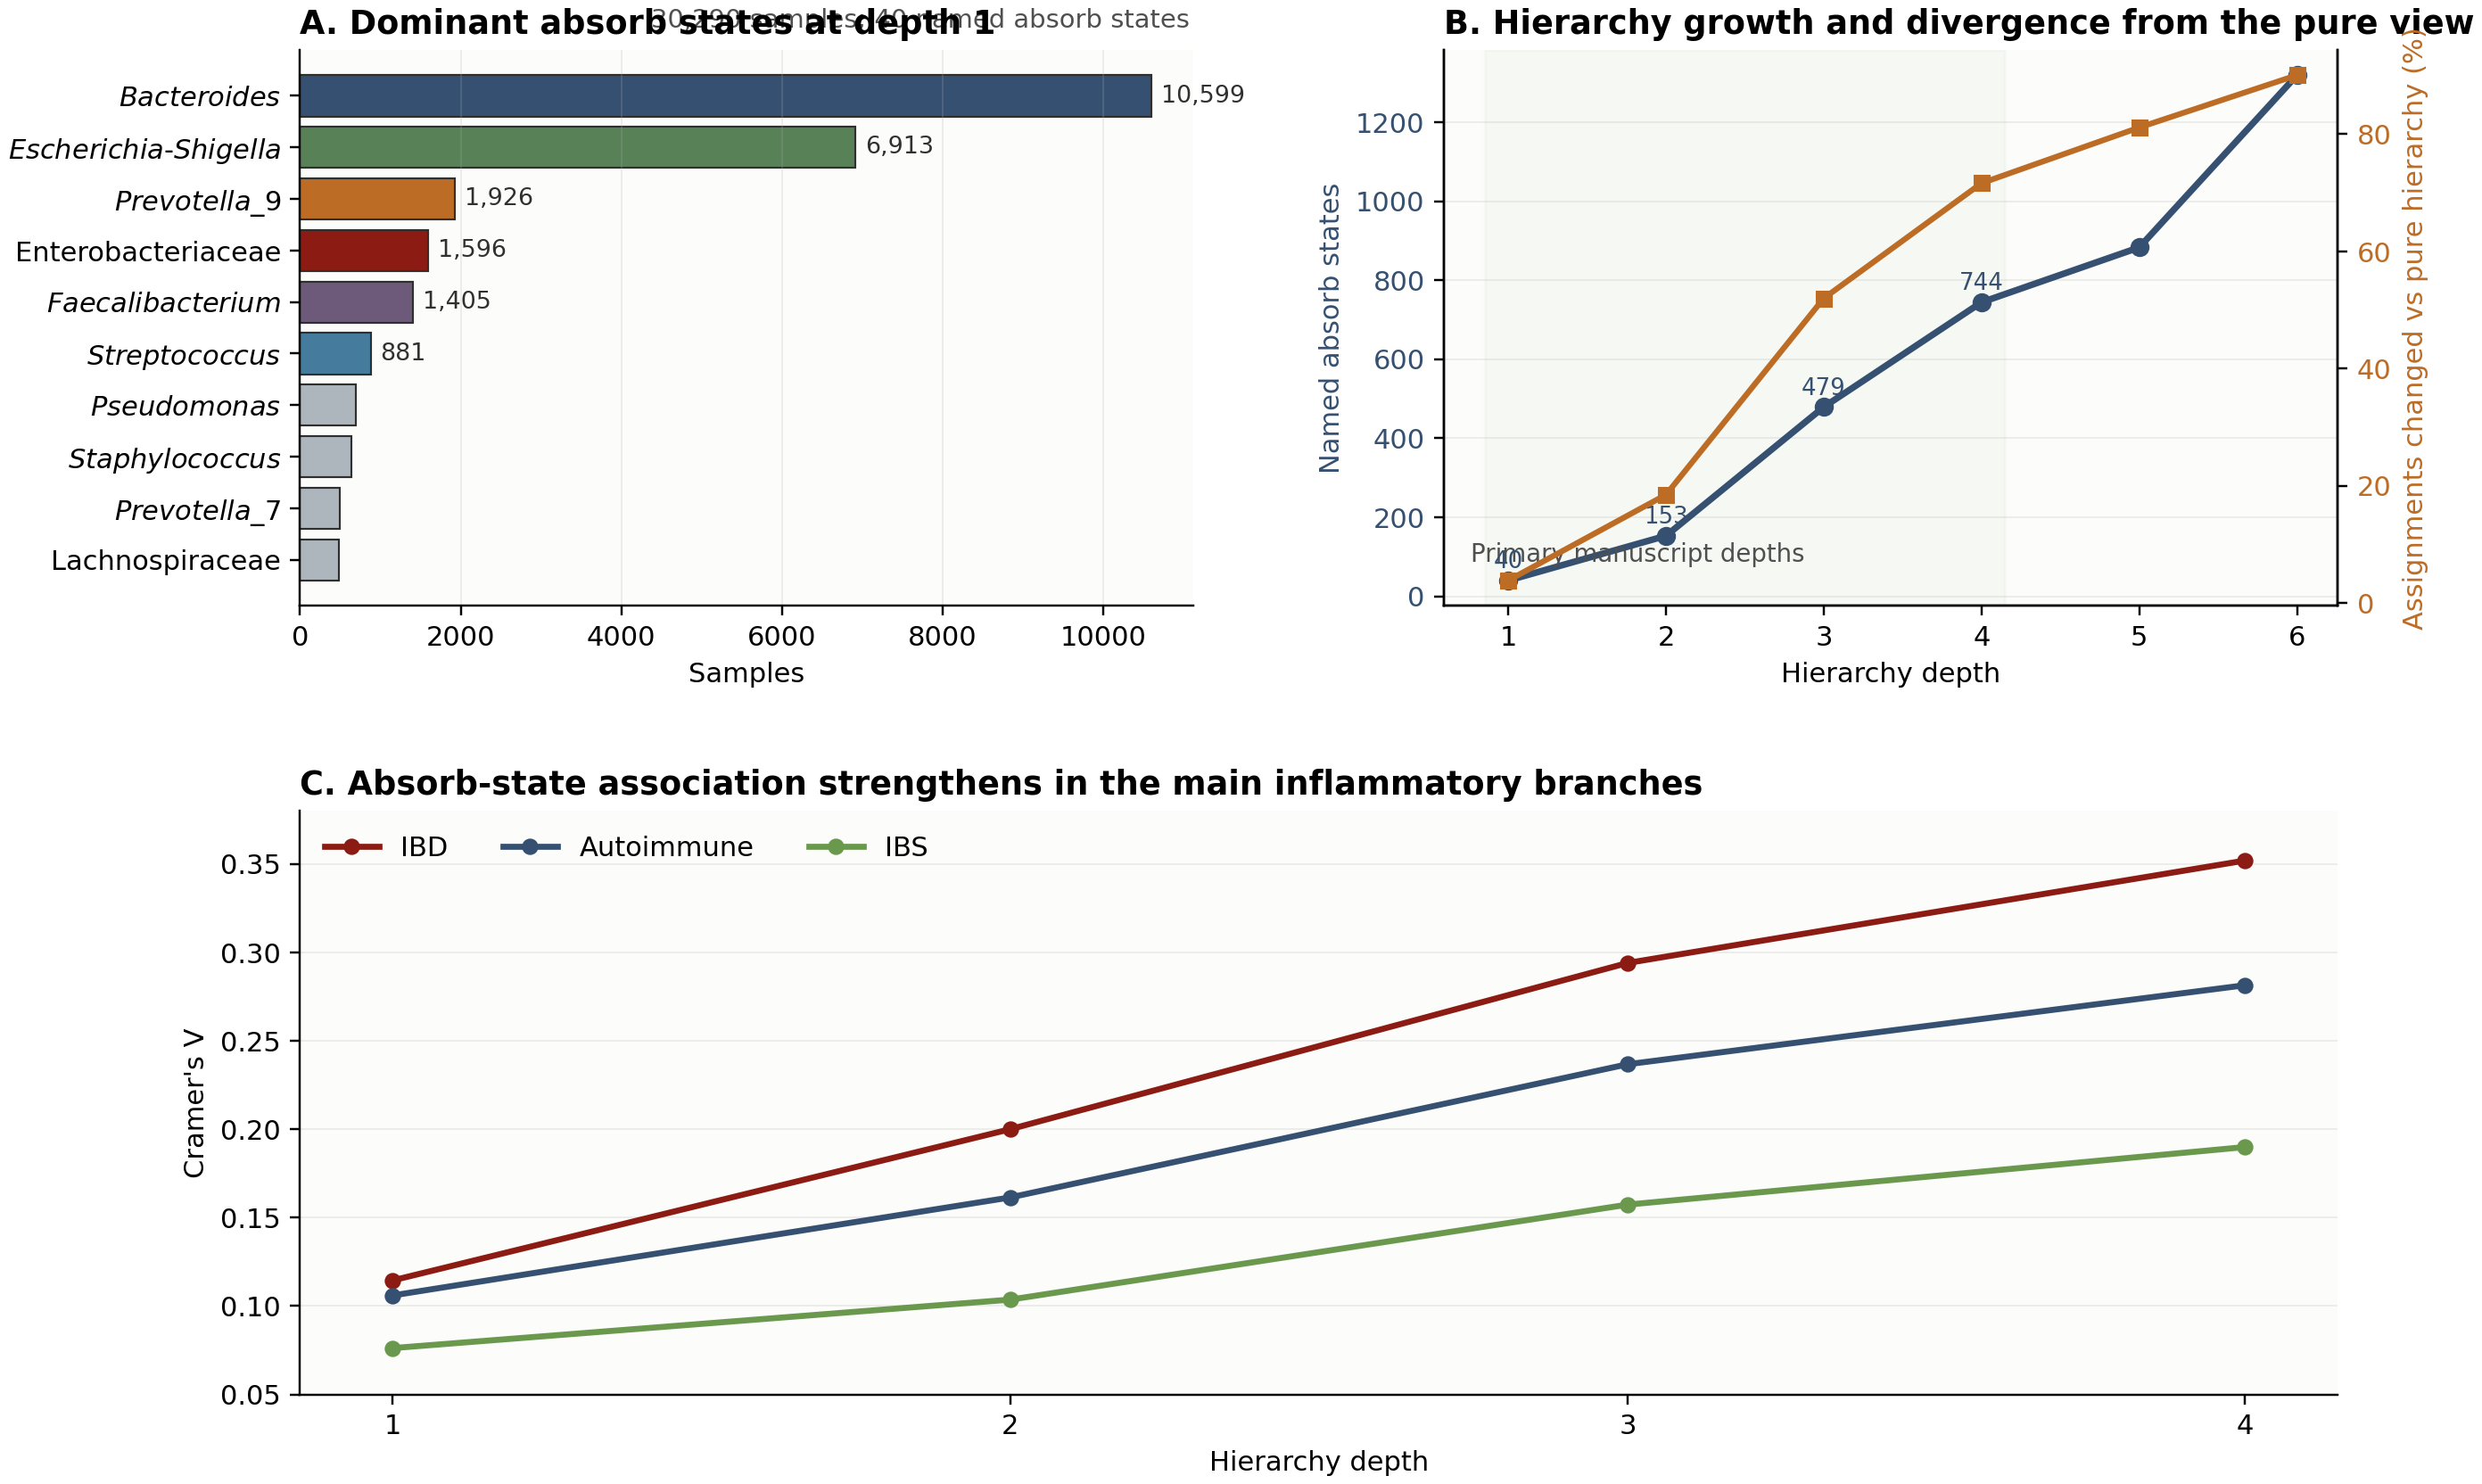
\includegraphics[width=0.98\linewidth,height=\textheight,keepaspectratio,alt={Absorb overview figure. Panel A shows the ten largest depth-1 absorb states in the AGP cohort. Panel B shows growth in the number of named absorb states across depths 1 to 6 together with the fraction of assignments that change relative to the pure hierarchy. Panel C shows Cramer's V across depths 1 to 4 for IBD, autoimmune disease, IBS, acid reflux, and seasonal allergies.}]{../assets/figures/FIGURE_2_absorb_overview.png}
\caption{Overview of the absorb hierarchy in the AGP discovery cohort. Panel A shows the largest named depth-1 absorb states. Panel B shows how the hierarchy expands from depth 1 to depth 6 together with the fraction of samples whose assignments differ from the pure hierarchy. Panel C shows the depthwise omnibus effect size, summarized by Cramer's V, for the three main-text phenotype branches together with two supplementary non-IBD examples.}
\end{figure}

The phenotype-wide absorb screen remained broad, with strong omnibus
signal across many outcomes at depths 1 through 4. We focus detailed
label-level interpretation on IBD, IBS, and autoimmune disease because
these branches combined clear depthwise growth in effect size with the
most stable frequentist and Bayesian lineage-level estimates.

\subsection{Inflammatory bowel disease
(IBD)}\label{inflammatory-bowel-disease-ibd}


IBD provides the most clinically grounded inflammatory phenotype in the
AGP screen. Landmark studies report reduced diversity, expansion of
Proteobacteria, and depletion of butyrate-associated commensals,
especially \emph{Faecalibacterium prausnitzii}
(\citeproc{ref-Frank2007_IBD}{Frank et al. 2007};
\citeproc{ref-Gevers2014_CD}{Gevers et al. 2014};
\citeproc{ref-LloydPrice2019_IBD}{Lloyd-Price et al. 2019};
\citeproc{ref-Sokol2008_Fprausnitzii}{Sokol et al. 2008};
\citeproc{ref-Manichanh2006_CD}{Manichanh et al. 2006}).

IBD produced the strongest absorb hierarchy in the cohort. In the
conservative adjusted depth-1 screen, the clearest frequentist signals
were enrichment of \taxon{Bacteroides} (adjusted OR 1.54, q =
8.1e-10), \taxon{Bifidobacterium} (adjusted OR 3.38, q =
2.2e-04), Enterobacterales (adjusted OR 3.23, q = 0.0016), and
Lachnospiraceae (adjusted OR 1.99, q = 0.0030), together with
depletion of \taxon{Prevotella\_9} (adjusted OR 0.44, q =
2.2e-04). The Bayesian layer recovered the same common-state picture,
but it also highlighted very rare enterobacterial states that were too
small for the conservative adjusted frequentist screen. In particular,
\taxon{Morganella} showed a Bayesian adjusted OR of 18.99
(95\% credible interval 10.15--35.53) and \taxon{Proteus} showed a
Bayesian adjusted OR of 3.40 (95\% credible interval 1.40--8.27), both
with near-complete posterior support for enrichment in IBD.

The value of the absorb hierarchy became even clearer at greater depth.
At depth 2, \taxon{Bacteroides}/Lachnospiraceae reached adjusted OR
3.21 (q = 2.6e-33), \taxon{Bacteroides}/[\emph{Eubacterium}]
\emph{eligens} group reached adjusted OR 22.50 (q = 5.0e-24), and
\taxon{Bacteroides}/Enterobacteriaceae reached adjusted OR 2.73 (q =
2.2e-04). At depth 3, the strongest lineage was
\taxon{Bacteroides}/Lachnospiraceae/\taxon{Alistipes} (adjusted OR
8.56, q = 1.5e-28), followed by
\taxon{Bacteroides}/\emph{[Eubacterium]\_eligens\_group}/Lachnospiraceae
(adjusted OR 22.50, q = 5.0e-24) and
\taxon{Bacteroides}/\taxon{Alistipes}/Lachnospiraceae (adjusted OR
5.95, q = 6.1e-15). At depth 4, the best supported lineage remained
\taxon{Bacteroides}/Lachnospiraceae/\taxon{Alistipes}/\taxon{Faecalibacterium}
(adjusted OR 5.53, q = 1.1e-07). For a biologist, the practical reading
is simple: the broad depth-1 \taxon{Bacteroides} state contains several
very different inflammatory sub-lineages, and the absorb policy keeps
those lineages named and interpretable instead of sending them into a
generic rare bucket.

\begin{figure}[H]
\centering
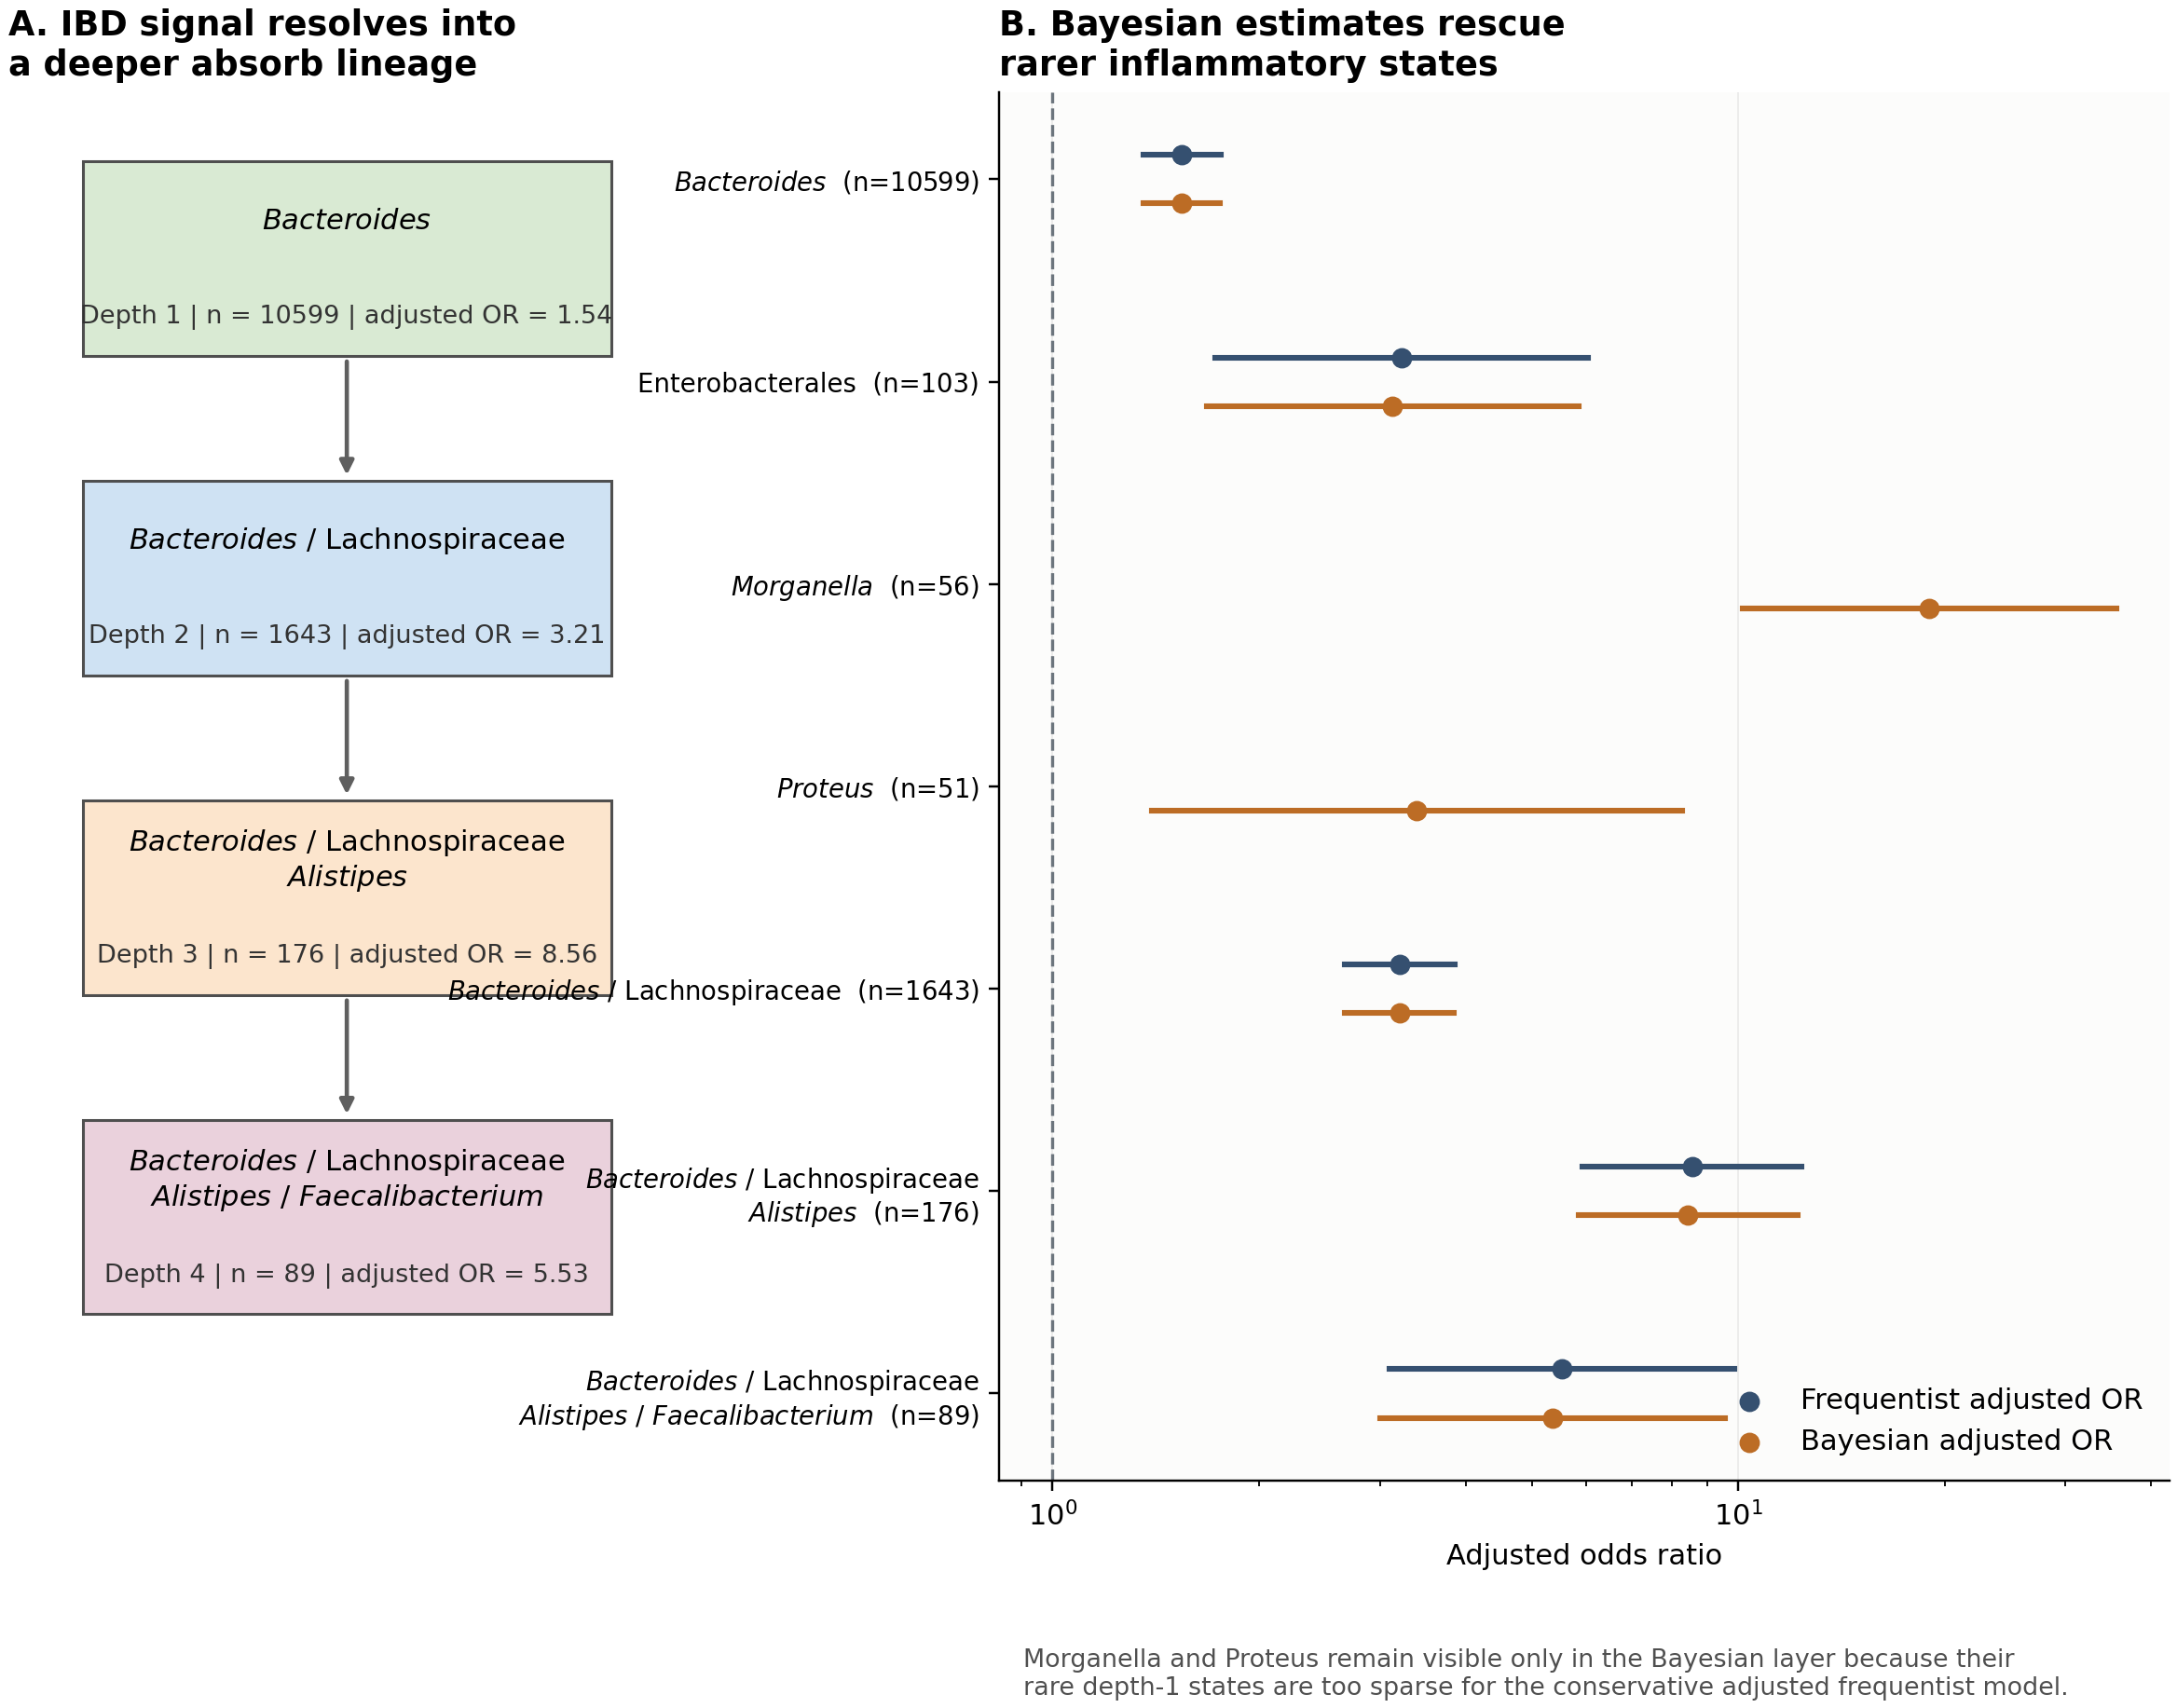
\includegraphics[width=0.98\linewidth,height=\textheight,keepaspectratio,alt={IBD absorb lineage figure. Panel A shows the progression from the broad depth-1 Bacteroides state to deeper Bacteroides-centered inflammatory lineages at depths 2 to 4. Panel B compares frequentist and Bayesian adjusted odds ratios for the main IBD lineage states and for rare enterobacterial states such as Morganella and Proteus.}]{../assets/figures/FIGURE_3_ibd_absorb_lineages.png}
\caption{IBD is the clearest lineage-resolved example in the absorb hierarchy. Panel A shows the progression from the broad depth-1 \taxon{Bacteroides} state to the depth-2 through depth-4 inflammatory lineages emphasized in the main text. Panel B compares frequentist and Bayesian adjusted odds ratios for representative IBD-associated states. The common lineages are supported by both frameworks, whereas rare enterobacterial states such as \taxon{Morganella} and \taxon{Proteus} remain visible mainly in the Bayesian analysis because the conservative adjusted frequentist model does not estimate stable coefficients for those sparse labels.}
\end{figure}

External validation asked two related but distinct questions. Rebuilt
cohort validation asked whether the absorb framework rediscovered
disease-associated dominant states when each external dataset was
analyzed independently. Frozen-transfer validation then asked whether
AGP-defined absorb states themselves could be assigned to external
samples and retain signal without rebuilding the hierarchy.

Across the completed inflammatory cohorts, rebuilt-cohort validation was
strongest in Halfvarson 2017, where the \texttt{IBD\_vs\_Healthy},
\texttt{Crohn\_vs\_Healthy}, and \texttt{UC\_vs\_Healthy} comparisons
all remained significant after multiple-testing correction. The leading
rebuilt labels differed across those contrasts but pointed to the same
broad inflammatory axis: depletion of \taxon{Segatella} sp. in pooled
IBD and Crohn disease together with enrichment of \taxon{Bacteroides}
\emph{dorei} in ulcerative colitis. PRJEB84421 provided narrower
support through
\texttt{OFG\_vs\_Healthy}, where a depth-2
\taxon{Faecalibacterium}\dcstsep\taxon{Bacteroides} lineage was depleted
(q = 0.019). By contrast, rebuilt \texttt{IBD\_vs\_Healthy} in HMP2 and
rebuilt \texttt{Crohn\_vs\_Healthy} in Gevers 2014 remained directional
but did not retain BH-significant absorb states, which is not
surprising given repeated sampling, substantial clinical heterogeneity,
and the more specialized ecology of those cohorts.

Frozen transfer was stricter but still informative. Halfvarson remained
clearly positive when samples were mapped directly onto AGP-defined
states: pooled IBD, Crohn, and UC comparisons all retained q < 0.001,
with the transferred signal centered on enriched \taxon{Bacteroides}
states and depleted \taxon{Faecalibacterium}-linked states. After
explicitly coding pooled HMP2 inflammatory bowel disease as one case
label, HMP2 also retained a weaker but significant depth-2 transferred
\taxon{Bacteroides}\dcstsep\taxon{Faecalibacterium} depletion in
\texttt{IBD\_vs\_Healthy} (q = 0.027). Gevers 2014 and PRJEB84421 both
mapped well into the AGP hierarchy but did not retain BH-significant
transferred states, and the current Jacobs IBS cohort was likewise
directional at most. We therefore interpret the present external data as
strongest support for inflammatory framework reproducibility, with exact
label portability clearly demonstrated in Halfvarson and supported more
selectively in pooled HMP2 (Figure 4; Supplementary Table S4).

\begin{figure}[H]
\centering
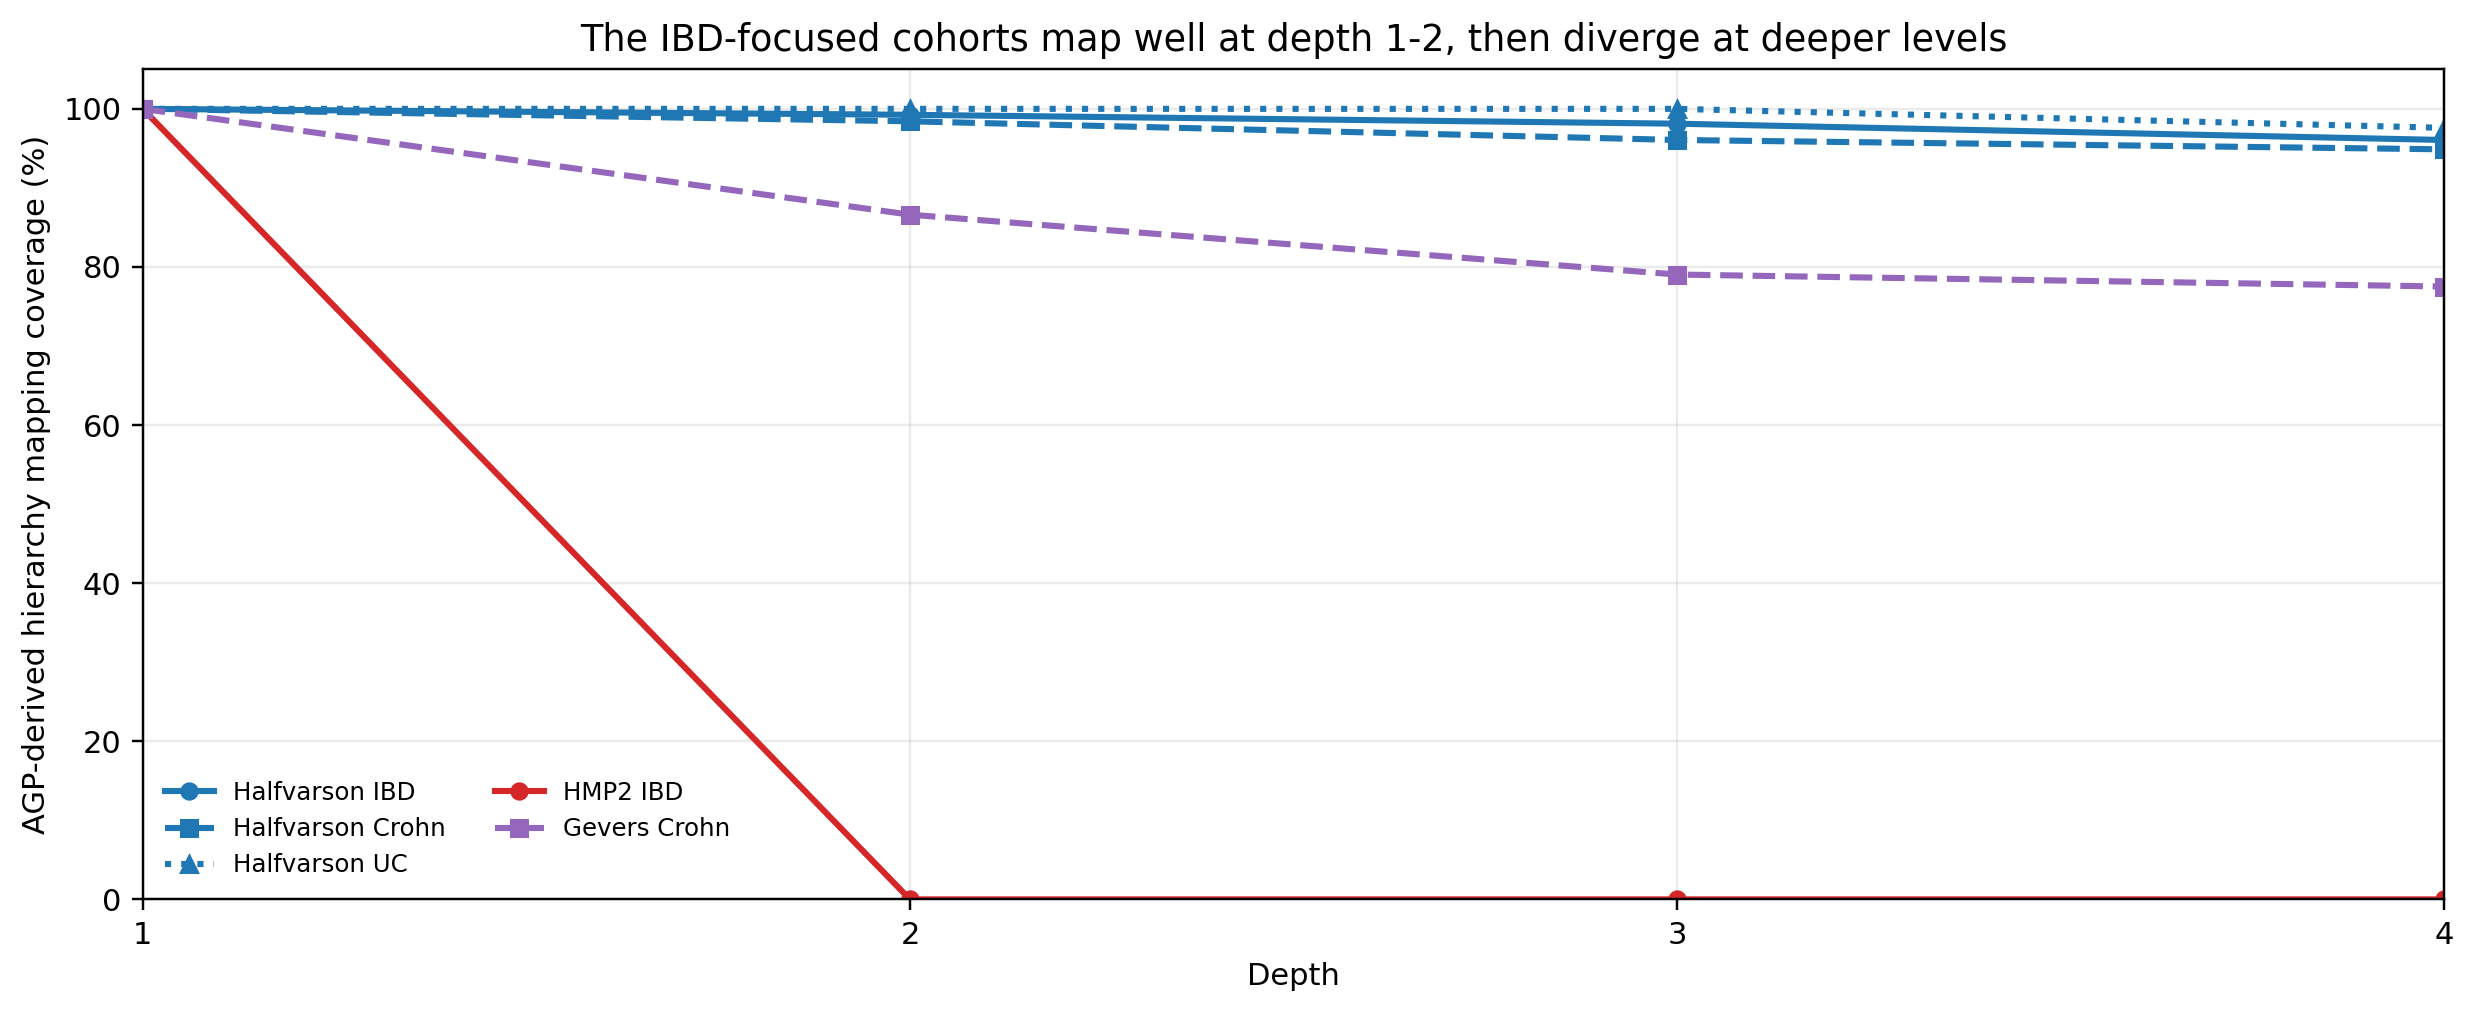
\includegraphics[width=0.98\linewidth,height=\textheight,keepaspectratio,alt={External validation comparison figure. Panel A compares the strongest BH-adjusted signal recovered for each key cohort-comparison under rebuilt-cohort absorb validation and under frozen AGP transfer validation. Panel B shows frozen-transfer mapping coverage across depths 1 to 4 for the same comparisons. Halfvarson stays positive in both modes, HMP2 retains a weaker transferred depth-2 signal, and the other cohorts map into the hierarchy but lose exact-state significance under the frozen transfer test.}]{../assets/figures/FIGURE_4_external_validation_modes.png}
\caption{External validation separates framework reproducibility from
exact label portability. Panel A compares the strongest BH-adjusted
signal recovered for each key cohort-comparison under rebuilt-cohort
absorb validation and under frozen AGP transfer validation. Rebuilt
cohort validation is broader, whereas frozen transfer is stricter and
therefore a better test of whether AGP-derived labels themselves can be
reused across studies. Panel B shows frozen-transfer mapping coverage
across depths 1 to 4 for the same comparisons. Halfvarson remains
strong in both modes, PRJEB84421 contributes narrower rebuilt
inflammatory support, HMP2 provides a weaker pooled IBD transfer signal
after explicit case coding, and the remaining cohorts map into the
hierarchy without equally strong corrected transferred associations.}
\end{figure}

These IBD results align well with the established literature. The
classic IBD story is not that one taxon always dominates, but that
protective obligate anaerobes are lost while inflammatory facultative
taxa expand (\citeproc{ref-Frank2007_IBD}{Frank et al. 2007};
\citeproc{ref-Gevers2014_CD}{Gevers et al. 2014};
\citeproc{ref-LloydPrice2019_IBD}{Lloyd-Price et al. 2019};
\citeproc{ref-Sokol2008_Fprausnitzii}{Sokol et al. 2008};
\citeproc{ref-Sartor2008_IBD}{Sartor 2008}). The absorb DCST analysis
compresses that pattern into an interpretable hierarchy: a broad
\taxon{Bacteroides} background, inflammatory
\taxon{Bacteroides}-centered lineages at greater depth, and a small set
of rare enterobacterial states marking more severe dysbiosis.

\subsection{Irritable bowel syndrome
(IBS)}\label{irritable-bowel-syndrome-ibs}


IBS provides a useful secondary test of the framework because its gut
microbiome signal is typically subtler than in overt inflammatory bowel
disease
(\citeproc{ref-Pittayanon2019_IBS}{Pittayanon et al. 2019};
\citeproc{ref-Dinan2015_IBS}{Dinan and Cryan 2015};
\citeproc{ref-Cryan2012_gutbrain}{Cryan and Dinan 2012}). In the absorb
hierarchy, IBS showed a moderate but internally consistent shift toward
enterobacterial dominance. At depth 1,
\taxon{Escherichia-Shigella} was enriched in IBS (adjusted OR 1.24, q =
0.002), while \taxon{Staphylococcus}, \taxon{Faecalibacterium}, and
\taxon{Prevotella\_9} were depleted. At depth 2, two
\taxon{Escherichia-Shigella}/\taxon{Bacteroides}-centered states
remained significant, and by depth 3 the clearest surviving frequentist
signal was an
\taxon{Escherichia-Shigella}/\taxon{Bacteroides}/Lachnospiraceae
lineage (adjusted OR 1.78, q = 0.018).

The Bayesian follow-up preserved the same ecological pattern at greater
depth, with strong posterior support for depletion of
\taxon{Faecalibacterium}- and \taxon{Prevotella\_9}-linked states and
for enrichment of deeper
\taxon{Escherichia-Shigella}/\taxon{Bacteroides}/Lachnospiraceae
lineages even when the frequentist q-values became sparse. Biologically,
the IBS branch therefore reads as a milder version of inflammatory
dominance shift rather than as a fully distinct ecological program,
which is compatible with the current IBS literature
(\citeproc{ref-Pittayanon2019_IBS}{Pittayanon et al. 2019};
\citeproc{ref-Tap2017_IBS}{Tap et al. 2017}).

\subsection{Autoimmune diseases}\label{autoimmune-diseases}


The AGP autoimmune phenotype is an umbrella label rather than a single
disease and therefore requires more cautious interpretation than IBD.
Even so,
autoimmune disease is an important category because the literature
repeatedly links loss of immune-regulatory commensals and expansion of
pathobionts to altered Treg/Th17 balance
(\citeproc{ref-Scher2013_Prevotella_RA}{Scher et al. 2013};
\citeproc{ref-Atarashi2013_Clostridia_Treg}{Atarashi et al. 2013};
\citeproc{ref-DeLuca2019_autoimmune}{De Luca and Shoenfeld 2019};
\citeproc{ref-Vatanen2018_T1D}{Vatanen et al. 2018}).

Autoimmune disease showed an absorb pattern that was clearly
inflammatory but more heterogeneous than IBD. At depth 1, the dominant
signals were enrichment of \taxon{Bacteroides} (adjusted OR 1.40, q =
1.6e-12) together with depletion of \taxon{Prevotella\_9},
\taxon{Streptococcus}, \taxon{Faecalibacterium}, and
\taxon{Staphylococcus}. At depth 2, the hierarchy sharpened around
\taxon{Bacteroides}-centered lineages:
\taxon{Bacteroides}/Lachnospiraceae reached adjusted OR 2.15 (q =
5.1e-22), \taxon{Bacteroides}/[\emph{Eubacterium}]
\emph{eligens\_group} reached adjusted OR 21.95 (q = 3.2e-20), and
\taxon{Bacteroides}/\taxon{Alistipes} reached adjusted OR 1.70 (q =
2.5e-05). The same branch continued deeper, with
\taxon{Bacteroides}/Lachnospiraceae/\taxon{Alistipes} reaching adjusted
OR 5.52 (q = 3.9e-21) at depth 3 and
\taxon{Bacteroides}/Lachnospiraceae/\taxon{Alistipes}/\taxon{Faecalibacterium}
remaining significant at depth 4 (adjusted OR 3.44, q = 6.1e-05).

The Bayesian analysis again helped mostly at the deeper levels. It
supported the same major \taxon{Bacteroides}-centered lineages as the
frequentist analysis, but it also retained support for additional depth-4
states such as
\taxon{Bacteroides}/\taxon{Akkermansia}/Lachnospiraceae/\taxon{Faecalibacterium}
and depleted
\taxon{Bacteroides}/\taxon{Faecalibacterium}/Lachnospiraceae/\taxon{Agathobacter}
states that no longer crossed the conventional q-value threshold. The
biological reading is therefore similar to IBD but more cautious: this
umbrella phenotype appears to be enriched for an inflammatory
\taxon{Bacteroides}-centered ecology, yet the pooled autoimmune label is
too broad to support one disease-specific mechanistic claim. The safest
interpretation is a shared inflammatory ecological axis rather than one
causal autoimmune taxon
(\citeproc{ref-Scher2013_Prevotella_RA}{Scher et al. 2013};
\citeproc{ref-Vatanen2018_T1D}{Vatanen et al. 2018};
\citeproc{ref-Atarashi2013_Clostridia_Treg}{Atarashi et al. 2013};
\citeproc{ref-DeLuca2019_autoimmune}{De Luca and Shoenfeld 2019}).

\section{Discussion}\label{general-discussion}

This absorb-based analysis makes two related points. First, merging very
small dominant states into larger named states is not a cosmetic change.
At depth 1, the absorb and pure views remain fairly close, but at
depths 2 through 4 the absorb policy preserves interpretable named
lineages instead of sending a growing fraction of samples into a
residual tail. Second, a parallel Bayesian layer is useful not because
it replaces standard testing, but because it keeps the ecological story
readable when states become rare. In practice, the frequentist and
Bayesian analyses agreed closely for common states, while the Bayesian
models stayed informative for smaller deeper states such as the rare IBD
enterobacterial branches.

Across the three phenotype branches developed in the main text, the
biological pattern is coherent. IBD remains the strongest and
best-validated inflammatory branch,
anchored by a broad \taxon{Bacteroides} background, a set of deeper
\taxon{Bacteroides}-centered inflammatory lineages, and rare
enterobacterial states that likely mark more severe dysbiosis. IBS is
weaker but directionally similar, with a shift toward
\taxon{Escherichia-Shigella}-centered states and away from
\taxon{Faecalibacterium}- and \taxon{Prevotella\_9}-linked states.
Autoimmune disease shows a parallel but broader inflammatory
\taxon{Bacteroides}-centered structure, which is plausible as a pooled
immune-dysregulation signal even though the AGP autoimmune label is too
heterogeneous for one disease-specific interpretation. For a biologist,
the practical message is that absorb DCSTs provide a simple way to name
recurrent ecological states and then ask whether those states are more
or less common in cases. Additional non-IBD branches were also detected,
but we treat them as supplementary exploratory examples rather than as
co-equal pillars of the main submission story.

Several limitations remain important. External validation now clarifies
both the promise and the current boundary of the approach. When
external cohorts are rebuilt independently, the absorb framework
reproduces the inflammatory branch most clearly in Halfvarson and more
narrowly in PRJEB84421, whereas HMP2 and Gevers contribute only mixed
or directional rebuilt evidence. When the AGP hierarchy is frozen and
transferred directly, Halfvarson remains clearly positive and pooled
HMP2 retains a weaker depth-2 transfer signal, but the other cohorts
mainly demonstrate mapping coverage rather than BH-significant label
transfer. We therefore interpret the current evidence as strong for
IBD-focused framework reproducibility, moderate for portability of
selected AGP-defined inflammatory states, and still limited for broad
claims about a universally transferable label dictionary. Exact label
transferability will need broader stool-based validation, especially
for IBS and any non-IBD extensions of this framework. AGP phenotypes are
also self-reported and cross-sectional, so
residual confounding, medication effects, and reverse causation remain
plausible. Those concerns are especially important for supplementary
non-IBD phenotypes. The current evidence nevertheless supports
the absorb framework as a biologically interpretable analysis layer and
motivates broader testing of its generalizability in independent
cohorts.

\section{Conclusion}\label{conclusion}

Taken together, these results support absorb DCSTs as a reproducible and
interpretable analysis layer for large gut microbiome cohorts. The
strongest current evidence lies in the inflammatory branches,
especially IBD, where the absorb hierarchy resolves a broad dominant
state into a set of biologically readable deeper lineages and where
cross-cohort support is already visible most clearly in Halfvarson and
more selectively in pooled HMP2 and PRJEB84421. The parallel Bayesian
analysis strengthens that picture by stabilizing rarer deeper states
without changing the main biological story. In this setting, absorb
DCSTs provide a practical way to move from high-dimensional abundance
tables to sample-level ecological labels that biologists can read and
compare directly. Secondary IBS and autoimmune results suggest that the
same framework can extend beyond the anchor IBD branch, while broader
non-IBD examples are best treated as supplementary and
hypothesis-generating until stronger external support is available.

\section{Data and Code
Availability}\label{data-and-code-availability}

The manuscript source and paper assets are maintained in the public
\texttt{linf} repository: \url{https://github.com/pgajer/linf}. The
project-specific discovery and follow-up runners are maintained in the
public \texttt{gut\_microbiome} repository:
\url{https://github.com/pgajer/gut_microbiome}. The discovery analysis
used the American Gut Project stool cohort (\texttt{PRJEB11419})
through PRIME-derived species-level abundance tables. The absorb
discovery hierarchy was generated with
\texttt{run\_agp\_absorb\_depthscan.R}, and the phenotype-specific
frequentist/Bayesian follow-up was generated with
\texttt{run\_absorb\_label\_followup.R}. External validation assets were
generated with
\texttt{run\_external\_case\_control\_validation\_absorb.R} and
\texttt{run\_external\_case\_control\_validation\_frozen\_agp.R}.
PRIME-derived HMP2 input exports were generated with
\texttt{export\_prime\_project\_validation\_inputs.py}. Supplementary
materials for the present manuscript summarize phenotype definitions
and sample counts, the pure-versus-absorb depth-change summary,
selected reference analyses retained outside the main text, and the
cross-cohort rebuilt-versus-frozen validation comparison.

\section{Funding}\label{funding}

\paperfundingnote

\section{Competing Interests}\label{competing-interests}

The authors declare no competing interests.

\section{Acknowledgments}\label{acknowledgments}

We thank the participants and investigators of the American Gut Project,
HMP2 / IBDMDB, PRJEB84421, Halfvarson 2017, and Gevers 2014 for making
these cohort resources available, and we thank the PRIME project context
that made the large-scale gut screen feasible.

\section*{References}\label{references}
\addcontentsline{toc}{section}{References}

\protect\phantomsection\label{refs}
\begin{CSLReferences}{1}{0}
\bibitem[\citeproctext]{ref-Atarashi2013_Clostridia_Treg}
Atarashi, Koji, Taira Tanoue, Keiji Oshima, et al. 2013. {``Treg
Induction by a Rationally Selected Mixture of {C}lostridia Strains from
the Human Microbiota.''} \emph{Nature} 500: 232--36.
\url{https://doi.org/10.1038/nature12331}.

\bibitem[\citeproctext]{ref-BenjaminiHochberg1995}
Benjamini, Yoav, and Yosef Hochberg. 1995. {``Controlling the False
Discovery Rate: A Practical and Powerful Approach to Multiple
Testing.''} \emph{Journal of the Royal Statistical Society Series B} 57:
289--300. \url{https://doi.org/10.1111/j.2517-6161.1995.tb02031.x}.

\bibitem[\citeproctext]{ref-Budden2017_gutlung}
Budden, Kurtis F, Shaan L Gellatly, David L A Wood, et al. 2017.
{``Emerging Pathogenic Links Between Microbiota and the Gut--Lung
Axis.''} \emph{Nature Reviews Microbiology} 15: 55--63.
\url{https://doi.org/10.1038/nrmicro.2016.142}.

\bibitem[\citeproctext]{ref-Cani2007_endotoxemia}
Cani, Patrice D, Jacques Amar, Miguel A Iglesias, et al. 2007.
{``Metabolic Endotoxemia Initiates Obesity and Insulin Resistance.''}
\emph{Diabetes} 56: 1761--72. \url{https://doi.org/10.2337/db06-1491}.

\bibitem[\citeproctext]{ref-Cryan2012_gutbrain}
Cryan, John F, and Timothy G Dinan. 2012. {``Mind-Altering
Microorganisms: The Impact of the Gut Microbiota on Brain and
Behaviour.''} \emph{Nature Reviews Neuroscience} 13: 701--12.
\url{https://doi.org/10.1038/nrn3346}.

\bibitem[\citeproctext]{ref-DeSouza2021_GERD}
D'Souza, S M, K Houston, L Keenan, B S Yoo, P J Parekh, and D A Johnson.
2021. {``Role of Microbial Dysbiosis in the Pathogenesis of Esophageal
Mucosal Disease: A Paradigm Shift from Acid to Bacteria?''} \emph{World
Journal of Gastroenterology} 27: 2054--72.
\url{https://doi.org/10.3748/wjg.v27.i18.2054}.

\bibitem[\citeproctext]{ref-DeLuca2019_autoimmune}
De Luca, F, and Y Shoenfeld. 2019. {``The Microbiome in Autoimmune
Diseases.''} \emph{Clinical and Experimental Immunology} 195: 74--85.
\url{https://doi.org/10.1111/cei.13158}.

\bibitem[\citeproctext]{ref-Deshpande2018_esophageal}
Deshpande, N P, S M Riordan, N Castaño-Rodríguez, M R Wilkins, and N O
Kaakoush. 2018. {``Signatures Within the Esophageal Microbiome Are
Associated with Host Genetics, Age, and Disease.''} \emph{Microbiome} 6:
227. \url{https://doi.org/10.1186/s40168-018-0611-4}.

\bibitem[\citeproctext]{ref-Dinan2015_IBS}
Dinan, Timothy G, and John F Cryan. 2015. {``Irritable Bowel Syndrome: A
Microbiome-Gut-Brain Axis Disorder?''} \emph{Neurogastroenterology and
Motility} 27: 445--55. \url{https://doi.org/10.1111/nmo.12520}.

\bibitem[\citeproctext]{ref-Everard2013_Akkermansia}
Everard, Amandine, Clara Belzer, Lucie Geurts, et al. 2013.
{``Cross-Talk Between \emph{{A}kkermansia Muciniphila} and Intestinal
Epithelium Controls Diet-Induced Obesity.''} \emph{Proceedings of the
National Academy of Sciences} 110: 9066--71.
\url{https://doi.org/10.1073/pnas.1219451110}.

\bibitem[\citeproctext]{ref-Forslund2015_metformin}
Forslund, Kristoffer, Falk Hildebrand, Trine Nielsen, et al. 2015.
{``Disentangling Type 2 Diabetes and Metformin Treatment Signatures in
the Human Gut Microbiota.''} \emph{Nature} 528: 262--66.
\url{https://doi.org/10.1038/nature15766}.

\bibitem[\citeproctext]{ref-Frank2007_IBD}
Frank, Daniel N, April L St Amand, Robert A Feldman, et al. 2007.
{``Molecular-Phylogenetic Characterization of Microbial Community
Imbalances in Human Inflammatory Bowel Diseases.''} \emph{Proceedings of
the National Academy of Sciences} 104: 13780--85.
\url{https://doi.org/10.1073/pnas.0706625104}.

\bibitem[\citeproctext]{ref-Gevers2014_CD}
Gevers, Dirk, Subra Kugathasan, Lee A Denson, et al. 2014. {``The
Treatment-Naive Microbiome in New-Onset {C}rohn's Disease.''} \emph{Cell
Host and Microbe} 15: 382--92.
\url{https://doi.org/10.1016/j.chom.2014.02.005}.

\bibitem[\citeproctext]{ref-Gorenshtein2025_migraine}
Gorenshtein, Alon, Kamel Shihada, Liron Leibovitch, Tom Liba, and Avner
Goren. 2025. {``The Association Between Migraine and Gut Microbiota: A
Systematic Review.''} \emph{Acta Neurologica Belgica} 125: 977--87.
\url{https://doi.org/10.1007/s13760-025-02779-y}.

\bibitem[\citeproctext]{ref-Horn2022_Prevotella_lung}
Horn, Kadi J, Melissa A Schopper, Zoe G Drigot, and Sarah E Clark. 2022.
{``Airway \emph{{P}revotella} Promote {TLR2}-Dependent Neutrophil
Activation and Rapid Clearance of \emph{{S}treptococcus Pneumoniae} from
the Lung.''} \emph{Nature Communications} 13: 3321.
\url{https://doi.org/10.1038/s41467-022-31074-0}.

\bibitem[\citeproctext]{ref-Hoskinson2023_allergy}
Hoskinson, C L, D L Y Dai, K L Del Bel, et al. 2023. {``Delayed Gut
Microbiota Maturation in the First Year of Life Is a Hallmark of
Pediatric Allergic Disease.''} \emph{Nature Communications} 14: 4785.
\url{https://doi.org/10.1038/s41467-023-40336-4}.

\bibitem[\citeproctext]{ref-Hua2016_AGP_allergy}
Hua, Xinmin, James J Goedert, Angela Pu, Guoqin Yu, and Jianxin Shi.
2016. {``Allergy Associations with the Adult Fecal Microbiota: Analysis
of the {A}merican {G}ut {P}roject.''} \emph{EBioMedicine} 3: 172--79.
\url{https://doi.org/10.1016/j.ebiom.2015.11.038}.

\bibitem[\citeproctext]{ref-Jie2017_ASCVD}
Jie, Zhuye, Huihua Xia, Shi-Long Zhong, et al. 2017. {``The Gut
Microbiome in Atherosclerotic Cardiovascular Disease.''} \emph{Nature
Communications} 8: 845.
\url{https://doi.org/10.1038/s41467-017-00900-1}.

\bibitem[\citeproctext]{ref-Kappeter2023_migraine_FMT}
Kappéter, Ágnes, Dávid Sipos, Adorján Varga, et al. 2023. {``Migraine as
a Disease Associated with Dysbiosis and Possible Therapy with Fecal
Microbiota Transplantation.''} \emph{Microorganisms} 11: 2083.
\url{https://doi.org/10.3390/microorganisms11082083}.

\bibitem[\citeproctext]{ref-Karlsson2013_T2D_women}
Karlsson, Fredrik H, Valentina Tremaroli, Intawat Nookaew, et al. 2013.
{``Gut Metagenomics in {E}uropean Women with Normal, Impaired and
Diabetic Glucose Control.''} \emph{Nature} 498: 99--103.
\url{https://doi.org/10.1038/nature12198}.

\bibitem[\citeproctext]{ref-LeChatelier2013_richness}
Le Chatelier, Emmanuelle, Trine Nielsen, Junjie Qin, et al. 2013.
{``Richness of Human Gut Microbiome Correlates with Metabolic
Markers.''} \emph{Nature} 500: 541--46.
\url{https://doi.org/10.1038/nature12506}.

\bibitem[\citeproctext]{ref-Ley2006_obesity}
Ley, Ruth E, Peter J Turnbaugh, Samuel Klein, and Jeffrey I Gordon.
2006. {``Human Gut Microbes Associated with Obesity.''} \emph{Nature}
444: 1022--23. \url{https://doi.org/10.1038/4441022a}.

\bibitem[\citeproctext]{ref-LloydPrice2019_IBD}
Lloyd-Price, Jason, Cesar Arze, Ashwin N Ananthakrishnan, et al. 2019.
{``Multi-Omics of the Gut Microbial Ecosystem in Inflammatory Bowel
Diseases.''} \emph{Nature} 569: 655--62.
\url{https://doi.org/10.1038/s41586-019-1237-9}.

\bibitem[\citeproctext]{ref-Manichanh2006_CD}
Manichanh, Chaysip, Laurence Rigottier-Gois, Emmanuelle Bonnaud, et al.
2006. {``Reduced Diversity of Faecal Microbiota in {C}rohn's Disease
Revealed by a Metagenomic Approach.''} \emph{Gut} 55: 205--11.
\url{https://doi.org/10.1136/gut.2005.073817}.

\bibitem[\citeproctext]{ref-McDonald2018_AGP}
McDonald, Daniel, Embriette Hyde, Justine W Debelius, et al. 2018.
{``{A}merican {G}ut: An Open Platform for Citizen Science Microbiome
Research.''} \emph{mSystems} 3: e00031--18.
\url{https://doi.org/10.1128/mSystems.00031-18}.

\bibitem[\citeproctext]{ref-McDonald2024_GG2}
McDonald, Daniel, Yueyu Jiang, Metin Balaban, et al. 2024.
{``{G}reen{G}enes2 Unifies Microbial Data in a Single Reference Tree.''}
\emph{Nature Biotechnology} 42: 715--18.
\url{https://doi.org/10.1038/s41587-023-02009-5}.

\bibitem[\citeproctext]{ref-Pittayanon2019_IBS}
Pittayanon, Rapat, Jennifer T Lau, Yuhong Yuan, Grigorios I Leontiadis,
Frances Tse, Michael G Surette, and Paul Moayyedi. 2019. {``Gut
Microbiota in Patients with Irritable Bowel Syndrome: A Systematic
Review.''} \emph{Gastroenterology} 157: 97--108.
\url{https://doi.org/10.1053/j.gastro.2019.03.049}.

\bibitem[\citeproctext]{ref-Qin2012_T2D}
Qin, Junjie, Yingrui Li, Zhiming Cai, et al. 2012. {``A Metagenome-Wide
Association Study of Gut Microbiota in Type 2 Diabetes.''} \emph{Nature}
490: 55--60. \url{https://doi.org/10.1038/nature11450}.

\bibitem[\citeproctext]{ref-Quast2013_SILVA}
Quast, Christian, Elmar Pruesse, Pelin Yilmaz, et al. 2013. {``The
{SILVA} Ribosomal {RNA} Gene Database Project: Improved Data Processing
and Web-Based Tools.''} \emph{Nucleic Acids Research} 41: D590--96.
\url{https://doi.org/10.1093/nar/gks1219}.

\bibitem[\citeproctext]{ref-Sartor2008_IBD}
Sartor, R Balfour. 2008. {``Microbial Influences in Inflammatory Bowel
Diseases.''} \emph{Gastroenterology} 134: 577--94.
\url{https://doi.org/10.1053/j.gastro.2007.11.059}.

\bibitem[\citeproctext]{ref-Scher2013_Prevotella_RA}
Scher, Jose U, Andrew Sczesnak, Randy S Longman, et al. 2013.
{``Expansion of Intestinal \emph{{P}revotella Copri} Correlates with
Enhanced Susceptibility to Arthritis.''} \emph{eLife} 2: e01202.
\url{https://doi.org/10.7554/eLife.01202}.

\bibitem[\citeproctext]{ref-Schubert2014_CDI}
Schubert, Allison M, Matthew A M Rogers, Corrie Ring, et al. 2014.
{``Microbiome Data Distinguish Patients with \emph{{C}lostridium
Difficile} Infection and Non-\emph{{C}. Difficile}-Associated Diarrhea
from Healthy Controls.''} \emph{mBio} 5: e01021--14.
\url{https://doi.org/10.1128/mBio.01021-14}.

\bibitem[\citeproctext]{ref-Seekatz2014_FMT}
Seekatz, Anna M, Jorn Aas, Christine E Gessert, et al. 2014. {``Recovery
of the Gut Microbiome Following Fecal Microbiota Transplantation.''}
\emph{mBio} 5: e00893--14. \url{https://doi.org/10.1128/mBio.00893-14}.

\bibitem[\citeproctext]{ref-Sehgal2021_CDI}
Sehgal, Kanika, and Sahil Khanna. 2021. {``Gut Microbiome and
\emph{{C}lostridioides Difficile} Infection: A Closer Look at the
Microscopic Interface.''} \emph{Therapeutic Advances in
Gastroenterology} 14: 1756284821994736.
\url{https://doi.org/10.1177/1756284821994736}.

\bibitem[\citeproctext]{ref-Sokol2008_Fprausnitzii}
Sokol, Harry, Bernardo Pigneur, Laetitia Watterlot, et al. 2008.
{``\emph{{F}aecalibacterium Prausnitzii} Is an Anti-Inflammatory
Commensal Bacterium Identified by Gut Microbiota Analysis of {C}rohn
Disease Patients.''} \emph{Proceedings of the National Academy of
Sciences} 105: 16731--36. \url{https://doi.org/10.1073/pnas.0804812105}.

\bibitem[\citeproctext]{ref-Strachan1989_hygiene}
Strachan, D P. 1989. {``Hay Fever, Hygiene, and Household Size.''}
\emph{BMJ} 299: 1259--60.
\url{https://doi.org/10.1136/bmj.299.6710.1259}.

\bibitem[\citeproctext]{ref-Takeuchi2023_carbohydrate}
Takeuchi, Takeshi, Tetsuya Kubota, Yumiko Nakanishi, et al. 2023. {``Gut
Microbial Carbohydrate Metabolism Contributes to Insulin Resistance.''}
\emph{Nature} 621: 591--98.
\url{https://doi.org/10.1038/s41586-023-06466-x}.

\bibitem[\citeproctext]{ref-Tang2015_TMAO_CKD}
Tang, W H Wilson, Zeneng Wang, David J Kennedy, et al. 2015. {``Gut
Microbiota-Dependent Trimethylamine {N}-Oxide ({TMAO}) Pathway
Contributes to Both Development of Renal Insufficiency and Mortality
Risk in Chronic Kidney Disease.''} \emph{Circulation Research} 116:
448--55. \url{https://doi.org/10.1161/CIRCRESAHA.116.305360}.

\bibitem[\citeproctext]{ref-Tang2013_TMAO}
Tang, W H Wilson, Zeneng Wang, Bruce S Levison, et al. 2013.
{``Intestinal Microbial Metabolism of Phosphatidylcholine and
Cardiovascular Risk.''} \emph{New England Journal of Medicine} 368:
1575--84. \url{https://doi.org/10.1056/NEJMoa1109400}.

\bibitem[\citeproctext]{ref-Tap2017_IBS}
Tap, Julien, Muriel Derrien, Henrik Törnblom, Romain Brazeilles, Sonia
Cools-Portier, Joël Doré, Sanna Störsrud, Benjamin Le Nevé, and Magnus
Simrén. 2017. {``Identification of an Intestinal Microbiota Signature
Associated with Severity of Irritable Bowel Syndrome.''}
\emph{Gastroenterology} 152: 111--23.
\url{https://doi.org/10.1053/j.gastro.2016.09.049}.

\bibitem[\citeproctext]{ref-Trompette2014_fiber_asthma}
Trompette, Aurélien, Evan S Gollwitzer, Khyati Yadava, et al. 2014.
{``Gut Microbiota Metabolism of Dietary Fiber Influences Allergic Airway
Disease and Hematopoiesis.''} \emph{Nature Medicine} 20: 159--66.
\url{https://doi.org/10.1038/nm.3444}.

\bibitem[\citeproctext]{ref-Turnbaugh2006_energy}
Turnbaugh, Peter J, Ruth E Ley, Michael A Mahowald, Vincent Magrini,
Elaine R Mardis, and Jeffrey I Gordon. 2006. {``An Obesity-Associated
Gut Microbiome with Increased Capacity for Energy Harvest.''}
\emph{Nature} 444: 1027--31. \url{https://doi.org/10.1038/nature05414}.

\bibitem[\citeproctext]{ref-Vatanen2018_T1D}
Vatanen, Tommi, Eric A Franzosa, Randall Schwager, et al. 2018. {``The
Human Gut Microbiome in Early-Onset Type 1 Diabetes from the {TEDDY}
Study.''} \emph{Nature} 562: 589--94.
\url{https://doi.org/10.1038/s41586-018-0620-2}.

\bibitem[\citeproctext]{ref-Vaziri2013_CKD}
Vaziri, Nosratola D, Jakk Wong, Madeleine Pahl, et al. 2013. {``Chronic
Kidney Disease Alters Intestinal Microbial Flora.''} \emph{Kidney
International} 83: 308--15. \url{https://doi.org/10.1038/ki.2012.345}.

\bibitem[\citeproctext]{ref-Walters2014_meta_obesity}
Walters, William A, Zech Xu, and Rob Knight. 2014. {``Meta-Analyses of
Human Gut Microbes Associated with Obesity and {IBD}.''} \emph{FEBS
Letters} 588: 4223--33.
\url{https://doi.org/10.1016/j.febslet.2014.09.039}.

\bibitem[\citeproctext]{ref-Wang2024_GERD_MR}
Wang, K, S Wang, Y Chen, X Lu, D Wang, Y Zhang, W Pan, C Zhou, and D
Zou. 2024. {``Causal Relationship Between Gut Microbiota and Risk of
Gastroesophageal Reflux Disease: A Genetic Correlation and Bidirectional
{M}endelian Randomization Study.''} \emph{Frontiers in Immunology} 15:
1327503. \url{https://doi.org/10.3389/fimmu.2024.1327503}.

\bibitem[\citeproctext]{ref-Wang2011_TMAO}
Wang, Zeneng, Erin Klipfell, Brian J Bennett, et al. 2011. {``Gut Flora
Metabolism of Phosphatidylcholine Promotes Cardiovascular Disease.''}
\emph{Nature} 472: 57--63. \url{https://doi.org/10.1038/nature09922}.

\bibitem[\citeproctext]{ref-Zhu2016_TMAO_thrombosis}
Zhu, W, J C Gregory, E Org, et al. 2016. {``Gut Microbe-Generated
Trimethylamine {N}-Oxide from Dietary Choline Is Prothrombotic in
Subjects.''} \emph{Cell} 165: 111--24.
\url{https://doi.org/10.1016/j.cell.2016.02.011}.

\end{CSLReferences}

\end{document}
